\chapter{Performing Time Evolution of Matrix Product States}
A central component of Optimal Control is time evolution. In order to compute any optimal control sequence, it is crucial to have a fast and accurate time evolution algorithm. However, also the construction of the time evolution operator must be taken into account, as exponentiating a tensor spanning the entire system, such as most Hamiltonians, is no easy task. In fact, since the time evolution operator is constantly altered when optimizing control parameters, the time spent exponentiating the Hamiltonian must be taken into account of the total runtime. Thus, both an efficient time evolution algorithm and an efficient operator exponentiation is needed when performing optimal control.\\
Several algorithms for time evolving matrix product states exist, however, they all origin from the same ideas proposed in \cite{Vidal2003,Vidal2004}. The most widely used of these algorithms is the tDMRG algorithm, which gets its name from its similarity with the ground state search algorithm described in Section \ref{sec:DMRG}. The tDMRG algorithm has been utilized in several instances to simulate the dynamics of one-dimensional systems CITE, and it has even been previously used in conjunction with the CRAB algorithm to perform optimal control of the Superfluid to Mott-Insulator phase transition \cite{FrankBloch,Doria2011}.\\
Although the standard algorithms for time evolution are quite efficient, further improvements can be made to the algorithms when tailoring to the problem at hand. Therefore, a modified version of the tDMRG algorithm is proposed in Section \ref{sec:modTMDRG}, which directly utilizes the properties of the Bose-Hubbard Hamiltonian.


\section{The tDMRG Algorithm}
Consider the time evolution of a quantum state
\begin{equation}
	\ket{\psi (t)} = \hat{\mathcal{U}}(t) \ket{\psi (0)} \; ,
\end{equation}
where $\hat{\mathcal{U}}(t) = \e^{ - \im \hat{H} t }$ is the time evolution operator. 
Time evolution of a matrix product states is done in a manner similar to that of ground state search, as the bonds between the tensors are evolved rather than the tensors themselves. Thus, the time evolution operator must be decomposed into two-site tensors. The simplest realisation of this is achieved, when considering a Hamiltonian containing only nearest-neighbour interactions.
Assume the Hamiltonian is a sum of two-site operators of the form $\hat{H} = \sum_{n} \hat{h}^{[n , n+1]}$. One can decompose this into a sum over even and odd bonds
\begin{equation}
	\hat{H} = \hat{H}_{\mathrm{odd}} \; + \; \hat{H}_{\mathrm{even}} = \sum_{n \; \mathrm{odd}} \hat{h}^{[n , n+1]} \; + \; \sum_{n \; \mathrm{even}} \hat{h}^{[n , n+1]} \; .
\end{equation}  
Exponentiating the Hamiltonian is non-trivial due to the non-commutativity of the operators, $[ \hat{h}_{\mathrm{odd}}^{[n , n+1]} \; , \; \hat{h}_{\mathrm{even}}^{[n , n+1]} ] \neq 0$. Considering a small time slice, $\delta t$, the exponentiation can be achieved through the Trotter-Suzuki expansion \cite{Suzuki}. To first order this reads
\begin{equation}
	\e^{- \im \hat{H} \; \Delta t} = \e^{- \im \hat{H}_{\mathrm{odd}} \; \Delta t } \e^{- \im \hat{H}_{\mathrm{even}} \; \Delta t} \; + \; \;  \mathrm{O}(\Delta t^2) \; ,
\end{equation}
where the error is due to the non-commutativity of the bond Hamiltonians. Thus, the time evolution operator can be expressed as the product
\begin{equation}
	\hat{\mathcal{U}}(\Delta t) \approx \left( \prod_{n \; \mathrm{odd}} \hat{\mathcal{U}}^{[n,n+1]} (\Delta t) \right) \left( \prod_{n \; \mathrm{even}} \hat{\mathcal{U}}^{[n,n+1]} (\Delta t) \right) \; ,
\end{equation}
where
\begin{equation}
	\hat{\mathcal{U}}^{[n,n+1]} (\Delta t) = \e^{- \im \hat{h}^{[n , n+1]} \; \Delta t } \; .
\end{equation}
The result is an MPO performing an infinitesimal time step on the odd bonds, and another MPO evolving the even bonds. An illustration of this is shown in Figure \ref{fig:oddevenops}.
\begin{figure}[h!]
	\centering
	\begin{tikzpicture}[inner sep=1mm]
	\def \reldist {1.5};
	\def \numb {6};
	\def \wid {2}

	\foreach \i in  {1,...,\numb} {
		\node[tensor] (t\i) at (\i * \reldist, 0) {};
		\draw[-] (t\i) -- (\i * \reldist , -2.8);	
	};
	
	\foreach \i in {1,...,5} {
        \pgfmathtruncatemacro{\iplusone}{\i + 1};
        \draw[-] (t\i) -- (t\iplusone);
	};
	
	\foreach \i in {1,3,5} {
        \node[twositeop, minimum width= \wid cm] (op\i) at (\reldist*\i + \wid/2 -0.25,-1) {$\hat{\mathcal{U}}^{\mathrm{even}} (\Delta t)$};
	};
	
	\foreach \i in {2,4,6} {
        \node[twositeop, minimum width= \wid cm] (op\i) at (\reldist*\i + \wid/2 -0.25,-2) {$\hat{\mathcal{U}}^{\mathrm{odd}} (\Delta t)$};
	};	
	
	\node (dot1) at (0,0) {$\dots$};
	\node (dot2) at (\numb * \reldist + \reldist,0) {$\dots$};
	\draw[-] (t1) -- (dot1);
	\draw[-] (t\numb) -- (dot2);
	
	\draw[decoration={calligraphic brace,amplitude=10pt}, decorate, line width=1.25pt, xshift=-4pt, yshift=0pt]
(0, -2.5) -- (0,-0.5) node [black,midway,xshift=-0.6cm] 
{\large $\Delta t$};
	
\end{tikzpicture}
	\caption{\textit{Approximation of each time step $\delta t$ using a Trotter-Suzuki decomposition, such that the time evolution operator is expressed as a product of unitary two-site operators.}}
	\label{fig:oddevenops}
\end{figure}
The tDMRG algorithm describes the most efficient and accurate way of contracting the tensor network detailed in Figure \ref{fig:oddevenops}. The algorithm gets its name from its similarity with the DMRG algorithm detailed in Section \ref{sec:DMRG}. In fact, the merge and unmerge procedure of the two algorithms is completely identical, whereby they only differ in the steps of applying the operator and proceeding to the next site. The following procedure details a time evolution step of the $n$'th bond \cite{schollwock}.

\subsection{Infinitesimal time-step update for tDMRG}
\begin{enumerate}
\item
\textbf{Merge:} Contract tensors $M^{[n]}$ and $M^{[n+1]}$ over the bond $\alpha_{n}$ creating a two-site tensor $\Theta^{j_n , j_{n+1}}$.

\item
\textbf{Apply unitary:} The two-site time evolution operator, $\hat{\mathcal{U}}^{[n, n+1]}$, is applied to $\Theta^{j_n , j_{n+1}}$
\begin{equation}
	\tilde{\Theta}_{\alpha_{n-1} , \alpha_{n+1}}^{j_n , j_{n+1} } = \sum_{j_n ', j_{n+1}'} U^{j_n  j_{n+1} , j_n '  j_{n+1}'} \; \Phi_{\alpha_{n-1} , \alpha_{n+1}}^{j_n ', j_{n+1} ' } \; .
\end{equation}

\item
\textbf{Unmerge:} Reshape $\tilde{\Phi}_{\alpha_{n-1} , \alpha_{n+1}}^{j_n ', j_{n+1} '}$ to a matrix and decompose it through an SVD. Applying $\hat{\mathcal{U}}^{[n, n+1]}$ causes an increase in bond dimension, $D \rightarrow d^2 D$, which must be truncated by keeping only the $D$ largest singular values from the SVD. 

\item
\textbf{Progress:}  Next, the center cite of the MPS must be shifted by two, in order to update the next even (odd) bond. This is achieved by merging tensors $M^{[n+1]}$ and $M^{[n+2]}$ and performing a second SVD, while reshaping the resulting $U$-matrices to left-normalised tensors to retain the canonical form. The product of the second SVD must be truncated as well, however, no loss of information will occur, as the Schmidt rank of the matrix $S$ will be at most $D$ following the first SVD. 
\end{enumerate}
Following the procedure will leave the MPS in position for application ofthe unitary $\hat{\mathcal{U}}^{[n+2 , n+3]}$. The efficiency of the tDMRG algorithm also depends on the sequence in which bonds are evolved. A simple, yet effective way is iterating from left to right when evolving even bonds, while iterating right to left when evolving odd bonds. Thereby, the centered cite of the mixed-canonical form is moved continuously through the MPS, rather than having to be reset when reaching the end of the system.\\

Although the tDMRG algorithm is a very powerful algorithm, an even higher efficiency can be achieved when tailoring the algorithm to the problem. In this case the problem is optimal control of the Superfluid to Mott-Insulator transition. Thus, the Hamiltonian contains both nearest-neighbour and on-site terms. Furthermore, the Hamiltonian is time dependent, and it is continuously modified in the process of searching for optimal control parameters. The following algorithm is a modification of the tDMRG algorithm, which accommodates the requirements of performing optimal control.


\section{Modified Time Evolution Algorithm for Optimal Control}
\label{sec:modTMDRG}
In order to efficiently conduct optimal control of a Bose-Hubbard system, a slightly modified version of the tDMRG algorithm was employed. As the Hamiltonian is changing with every time step, one has to account for the time spent exponentiating the operators when considering the runtime of the algorithm. A general operator $\hat{W}$ can be exponentiated through the series expansion
\begin{equation}
	\exp \left( \hat{W} \right) = \sum_{k = 0}^{\infty} \frac{\hat{W}^k}{k!} = \hat{\mathds{1}} + \hat{W} \Bigl(  \hat{\mathds{1}} + \frac{\hat{W}}{2} \Bigl( \hat{\mathds{1}} + \frac{\hat{W}}{3} \Bigl( \ldots
\label{eq:exponentialSeries}
\end{equation}
The number of terms needed in the expansion to accurately describe the exponentiation depends on the operator. Performing the exponentiation through a series expansion is a relatively expensive operator. Therefore, it is crucial to find an easier way of constructing the time evolution operator.
One method is by considering the form of the Bose-Hubbard Hamiltonian. The most natural choice of control parameter is the lattice depth, $V_0$, as it is controllable experimentally. The lattice depth determines both the tunneling matrix element, $J$ (eq. \eqref{eq:BHparamJ}), and the interaction matrix element, $U$ (eq. \eqref{eq:BHparamU}), and has served as control parameter in other studies CITE.   
Unfortunately exponentiating the hopping terms of the Bose-Hubbard Hamiltonian was relatively high. Therefore, it was concluded that keeping $J$ fixed and using $U$ as the control parameter was the better option. Due to the diagonal form of the number operator, $\hat{n}_i$, the exponentiation of the interaction term can be built directly without the need for the series expansion of eq. \eqref{eq:exponentialSeries}.
However, simply exponentiating the different terms of the Bose-Hubbard Hamiltonian separately is not possible, as the operators do not commute. Therefore, one must expand the time evolution operator into its components through the Suzuki-Trotter expansion. To second order the Suzuki-Trotter expansion reads
\begin{equation}
	\exp\left(  ( \hat{V} + \hat{W}  ) \delta \right) = \exp\left(  \hat{V} \delta /2  \right) \exp\left(  \hat{W} \delta   \right) \exp\left(  \hat{V} \delta /2  \right) + O(\delta^3) \; . \label{eq:SuzukiTrotter}
\end{equation}
Once again, the error is due to the non-commutativity of operators. Thus, the time evolution operator can be divided into a sequence of tensors, where
\begin{align}
	\hat{\mathcal{U}}_{J}^{[i,i+1]} (\Delta t) &= \exp \left( -i J ( \hat{a}_{i}^{\dag} \hat{a}_{i+1} + \hat{a}_{i+1}^{\dag} \hat{a}_{i} ) \Delta t \right) \\
	\hat{\mathcal{U}}_{U}^{[i]} (\Delta t /2) &= \exp \left( -i \frac{U}{2} \hat{n}_i (\hat{n}_i -1) \Delta t /2 \right) \; .
\end{align}
\begin{figure}[h!]
	\centering
	\begin{tikzpicture}[inner sep=1mm]
\def \reldist {2};
\def \numb {4};
\def \wid {2.8};
\def \size {1.0};
\def \hi {0.8};
\def \vert {1.25};
\def \rad {0.4};

	
\foreach \i in  {1,...,\numb} {
	\node[tensor,minimum width= \size cm,minimum height= \size cm, rounded corners = 0.2cm] (A\i)
	at (\i * \reldist, 0) {$M^{[ \i ]}$};
	\draw[-] (A\i) -- (\i * \reldist , -4.7*\vert);	
};

\foreach \i in {1,...,3} {
    \pgfmathtruncatemacro{\iplusone}{\i + 1};
    \draw[-] (A\i) -- (A\iplusone);
};


\foreach \i in  {1,...,\numb} {
	\node[operator,minimum width= \hi cm,minimum height= \hi cm] (op\i)
	at (\i * \reldist, -\vert )
	{\scriptsize $\hat{\mathcal{U}}_{U}^{[ \i ]}$};	
};

\foreach \i in {1,...,\numb} {
	\pgfmathtruncatemacro{\j}{\i + 1};
    \node[twositeop, minimum width= \wid cm,minimum height= \hi cm,rounded corners = \rad cm] (eop\i)
    at (\reldist*\i + \reldist/2, {-2*\vert - Mod(\j,2) *\vert })
    {\small $\hat{\mathcal{U}}_{J}^{[ \i , \j ]} $};
};

\foreach \i in  {1,...,\numb} {
	\node[operator,minimum width= \hi cm,minimum height= \hi cm] (op\i)
	at (\i * \reldist, -4*\vert )
	{\scriptsize $\hat{\mathcal{U}}_{U}^{[ \i ]}$};	
};




\draw[decoration={calligraphic brace,amplitude=10pt}, decorate, line width=1.25pt, xshift=-4pt, yshift=0pt]
(0, -4*\vert -0.4) -- (0,-0.8) node [black,midway,xshift=-0.6cm] 
{\large $\Delta t$};


	\node (dot2) at (\numb * \reldist + 2,0) {$\dots$};

	\draw[-] (A\numb) -- (dot2);
	
	
\end{tikzpicture}
	\caption{\textit{Tensor diagram depicting a single time step of the modified rDMRG algorithm. The time evolution operator has been subjected to a Suzuki-Trotter expansion as detailed in eq. \eqref{eq:SuzukiTrotter}. The tensors of the upper part of the network are contracted with the MPS while sweeping from left to right, whereas the lower part is applied with a right-to-left sweep.}}
	\label{fig:ModifiedTEBD}
\end{figure}
A single time step, $\Delta t$, using the expanded operator is represented diagrammatically in figure \ref{fig:ModifiedTEBD}. At first glance, the tensor network resulting from the Suzuki-Trotter expansion may seem rather extensive, however, it can be contracted in a very efficient manner. The upper part of the network is contracted in a left-to-right sweeping manner, where the position of the center cite, and thereby the normalisation of the MPS, is pushed to the right following each step. Likewise, the lower part of the network is contracted though a right-to-left sweep such that the MPS returns to its original form centered on the first site after applying the final operator. Thereby, the MPS is immediately ready for the subsequent time-propagation.\\
\begin{figure}[h!]
\centering % <-- add this
\begin{subfigure}[b]{0.4\textwidth}
	\caption{}  
  	\begin{tikzpicture}[inner sep=1mm]
\def \reldist {2};
\def \numb {4};
\def \wid {3.2};
\def \size {1.0};
\def \rad {0.5};



\node[tensorc,minimum width= \size cm,minimum height= \size cm, rounded corners = 0.2cm] (A1) at (1 * \reldist, 0) {$A^{[1]}$};

\node[tensorr,minimum width= \size cm,minimum height= \size cm, rounded corners = 0.2cm] (A2) at (2 * \reldist, 0) {$A^{[2]}$};

\node[tensorr,minimum width= \size cm,minimum height= \size cm, rounded corners = 0.2cm] (A3) at (3 * \reldist, 0) {$A^{[3]}$};

\node[tensorr,minimum width= \size cm,minimum height= \size cm, rounded corners = 0.2cm] (A4) at (4 * \reldist, 0) {$A^{[4]}$};

\foreach \i in  {1,...,\numb} {
	\draw[-] (A\i) -- (\i * \reldist , -8.5);	
};

\foreach \i in {1,...,3} {
    \pgfmathtruncatemacro{\iplusone}{\i + 1};
    \draw[-] (A\i) -- (A\iplusone);
};

\node[twositeop, minimum width= \wid cm,minimum height= \size cm,rounded corners = \rad cm] (fop1)
    at (\reldist*1 + \reldist/2,-1.5)
    {\small $\hat{\mathcal{U}}_{J}^{[1,2]}(\delta t /2)$};
    
\node[twositeop, minimum width= \wid cm,minimum height= \size cm,rounded corners = \rad cm] (fop3)
    at (\reldist*3 + \reldist/2,-1.5)
    {\small $\hat{\mathcal{U}}_{J}^{[3,4]}(\delta t /2)$};

\node[twositeop, minimum width= \wid cm,minimum height= \size cm,rounded corners = \rad cm] (fop2)
    at (\reldist*2 + \reldist/2,-3)
    {$\hat{\mathcal{U}}_{J}^{[2,3]}(\delta t /2)$};
	
	
\foreach \i in  {1,...,\numb} {
	\node[operator,minimum width= \size cm,minimum height= \size cm] (op\i)
	at (\i * \reldist, -4.5)
	{\scriptsize $\hat{\mathcal{U}}_{U}(\delta t)$};	
};

\node[twositeop, minimum width= \wid cm,minimum height= \size cm,rounded corners = \rad cm] (sop1)
    at (\reldist*1 + \reldist/2,-6)
    {\small $\hat{\mathcal{U}}_{J}^{[1,2]}(\delta t /2)$};
    
\node[twositeop, minimum width= \wid cm,minimum height= \size cm,rounded corners = \rad cm] (sop3)
    at (\reldist*3 + \reldist/2,-6)
    {\small $\hat{\mathcal{U}}_{J}^{[3,4]}(\delta t /2)$};

\node[twositeop, minimum width= \wid cm,minimum height= \size cm,rounded corners = \rad cm] (sop2)
    at (\reldist*2 + \reldist/2,-7.5)
    {$\hat{\mathcal{U}}_{J}^{[2,3]}(\delta t /2)$};



	\node (dot2) at (\numb * \reldist + 2.4,0) {$\dots$};
	\draw[-] (A\numb) -- (dot2);
	
	
\end{tikzpicture}
\end{subfigure}
\hspace{10mm}
\begin{subfigure}[b]{0.4\textwidth}
	\caption{}    
  	\begin{tikzpicture}[inner sep=1mm]
\def \reldist {2};
\def \numb {4};
\def \wid {3.2};
\def \size {1.0};
\def \rad {0.5};



\node[tensorc,minimum width= \size cm,minimum height= \size cm, rounded corners = 0.2cm] (A1) at (1 * \reldist, 0) {$A^{[1]}$};

\node[tensorr,minimum width= \size cm,minimum height= \size cm, rounded corners = 0.2cm] (A2) at (2 * \reldist, 0) {$A^{[2]}$};

\node[tensorr,minimum width= \size cm,minimum height= \size cm, rounded corners = 0.2cm] (A3) at (3 * \reldist, 0) {$A^{[3]}$};

\node[tensorr,minimum width= \size cm,minimum height= \size cm, rounded corners = 0.2cm] (A4) at (4 * \reldist, 0) {$A^{[4]}$};

\node[tensor,minimum width= \wid cm,minimum height= \size cm, rounded corners = 0.2cm] (AA) at (\reldist*1 + \reldist/2, 0) {$\Theta$};

\foreach \i in  {1,...,\numb} {
	\draw[-] (A\i) -- (\i * \reldist , -8.5);	
};

\foreach \i in {1,...,3} {
    \pgfmathtruncatemacro{\iplusone}{\i + 1};
    \draw[-] (A\i) -- (A\iplusone);
};

\node[twositeop, minimum width= \wid cm,minimum height= \size cm,rounded corners = \rad cm] (fop1)
    at (\reldist*1 + \reldist/2,-1.5)
    {\small $\hat{\mathcal{U}}_{J}^{[1,2]}(\delta t /2)$};
    
\node[twositeop, minimum width= \wid cm,minimum height= \size cm,rounded corners = \rad cm] (fop3)
    at (\reldist*3 + \reldist/2,-1.5)
    {\small $\hat{\mathcal{U}}_{J}^{[3,4]}(\delta t /2)$};

\node[twositeop, minimum width= \wid cm,minimum height= \size cm,rounded corners = \rad cm] (fop2)
    at (\reldist*2 + \reldist/2,-3)
    {$\hat{\mathcal{U}}_{J}^{[2,3]}(\delta t /2)$};
	
	
\foreach \i in  {1,...,\numb} {
	\node[operator,minimum width= \size cm,minimum height= \size cm] (op\i)
	at (\i * \reldist, -4.5)
	{\scriptsize $\hat{\mathcal{U}}_{U}(\delta t)$};	
};

\node[twositeop, minimum width= \wid cm,minimum height= \size cm,rounded corners = \rad cm] (sop1)
    at (\reldist*1 + \reldist/2,-6)
    {\small $\hat{\mathcal{U}}_{J}^{[1,2]}(\delta t /2)$};
    
\node[twositeop, minimum width= \wid cm,minimum height= \size cm,rounded corners = \rad cm] (sop3)
    at (\reldist*3 + \reldist/2,-6)
    {\small $\hat{\mathcal{U}}_{J}^{[3,4]}(\delta t /2)$};

\node[twositeop, minimum width= \wid cm,minimum height= \size cm,rounded corners = \rad cm] (sop2)
    at (\reldist*2 + \reldist/2,-7.5)
    {$\hat{\mathcal{U}}_{J}^{[2,3]}(\delta t /2)$};



	\node (dot2) at (\numb * \reldist + 2.4,0) {$\dots$};
	\draw[-] (A\numb) -- (dot2);
	
	
\end{tikzpicture}
\end{subfigure}
\\ % <-- add this
\vspace{5mm}
\begin{subfigure}[b]{0.4\textwidth}
	\caption{}    	
  	\begin{tikzpicture}[inner sep=1mm]
\def \reldist {2};
\def \numb {2};
\def \wid {3.2};
\def \size {1.0};
\def \rad {0.5};



\node[tensor,minimum width= \size cm,minimum height= \size cm, rounded corners = 0.2cm] (A1) at (1 * \reldist, 0) {$A^{[1]}$};

\node[tensor,minimum width= \size cm,minimum height= \size cm, rounded corners = 0.2cm] (A2) at (2 * \reldist, 0) {$A^{[2]}$};


\foreach \i in  {1,...,\numb} {
	\draw[-] (A\i) -- (\i * \reldist ,-2.5);	
};
   
\draw[-] (A1) -- (A2);    

\node[twositeop, minimum width= \wid cm,minimum height= \size cm,rounded corners = \rad cm] (fop2)
    at (\reldist*2 + \reldist/2, -1.5 )
    {$\hat{\mathcal{U}}_{J}^{[2,3]}(\delta t /2)$};
	
\node[operator,minimum width= \size cm,minimum height= \size cm] (op1)
	at ( \reldist, -1.5)
	{\scriptsize $\hat{\mathcal{U}}_{U}(\delta t)$};	

\draw[-,line width=0.8mm] (A1) -- (op1);

\node (dot2) at (\numb * \reldist + 1.4,0) {$\dots$};
\draw[-] (A\numb) -- (dot2);
	
	
\end{tikzpicture}
\end{subfigure}
\hspace{10mm}
\begin{subfigure}[b]{0.4\textwidth}
	\caption{}  
  	\begin{tikzpicture}[inner sep=1mm]
\def \reldist {1.5};
\def \numb {4};
\def \wid {2.3};
\def \size {1.0};
\def \hi {0.8};
\def \rad {0.4};
\def \vert {1.35};


\foreach \i in  {1,...,\numb} {
	\node[tensorr,minimum width= \size cm,minimum height= \size cm, rounded corners = 0.2cm] (A\i)
	at (\i * \reldist, 0) {$M^{[ \i ]}$};
	\draw[-] (A\i) -- (\i * \reldist , -2.5*\vert);	
};

\foreach \i in {1,...,3} {
    \pgfmathtruncatemacro{\iplusone}{\i + 1};
    \draw[-] (A\i) -- (A\iplusone);
};

\node[tensorl,minimum width= \size cm,minimum height= \size cm, rounded corners = 0.2cm] (L1) at (1 * \reldist, 0) {$M^{[1]}$};

\node[tensorl,minimum width= \size cm,minimum height= \size cm, rounded corners = 0.2cm] (L2) at (2 * \reldist, 0) {$M^{[2]}$};

\node[tensorc,minimum width= \size cm,minimum height= \size cm, rounded corners = 0.2cm] (C) at (3 * \reldist, 0) {$M^{[3]}$};


\foreach \i in  {1,...,\numb} {
	\draw[-] (A\i) -- (\i * \reldist , -2.6 *\vert);	
};

\draw[-,line width=0.8mm] (A3) -- (A4);

\foreach \i in  {3,...,\numb} {
	\node[operator,minimum width= \hi cm,minimum height= \hi cm] (op\i)
	at (\i * \reldist, -\vert)
	{\scriptsize $\hat{\mathcal{U}}_{U}^{[ \i ]}$};	
};

\foreach \i in {3} {
	\pgfmathtruncatemacro{\j}{\i + 1};
    \node[twositeop, minimum width= \wid cm,minimum height= \hi cm,rounded corners = \rad cm] (top\i)
    at (\reldist*\i + \reldist/2, -2*\vert)
    {\small $\hat{\mathcal{U}}_{J}^{[ \i , \j ]} $};
};


\node (dot2) at (\numb * \reldist + 1.4,0) {$\dots$};
\draw[-] (A\numb) -- (dot2);
	
	
\end{tikzpicture}
\end{subfigure}
\caption{\textit{Sequence of contractions for modified tDMRG algorithm during left to right sweep. Step \textbf{(i)}: MPS is centered on site 1. Tensors $M^{[1]}$ and $M^{[2]}$ are contracted. Step \textbf{(ii)}: Two-site tensor, $\Theta$, is contracted with operators in numbered sequence. The propagated two-site tensor is split using an SVD in step \textbf{(iii)}, followed by a contraction to the right. Lastly, in step \textbf{(iv)}, the two-site tensor of $M^{[2]}$ and $M^{[3]}$ is split using another SVD, whereby the center (and thereby the normalisation) is pushed to site 3.}}
\label{fig:TEBDContraction}
\end{figure}
The sequence of contractions of the left-to-right sweep is shown in figure \ref{fig:TEBDContraction}. The MPS is initially centered on the first tensor, while its remaining tensors are all right-normalised. By contracting the bonds marked with a bold line, the operators are efficiently applied to the MPS. In step (iii) the two-site tensor, $\Theta$, is split using an SVD, where the bond dimension of the tensors is truncated. This is crucial in order to maintain a reduced dimensionality, which would otherwise result in a significant increase in contraction time. In the final step (iv), the central cite of the MPS is moved to the start of the next two-site operator through another site merge and subsequent SVD. This step is exactly as in the original tDMRG algorithm. Thereby the normalisation of the MPS is "pushed" to the right and contained in a single site, which makes it easy to deal with in the end of the time evolution step.\\
As the center reaches the end of the MPS, the direction of the sweep is reversed. The right-to-left sweep is very similar to the sequence described above. The main difference is in the order of contractions, as the $\hat{\mathcal{U}}_{J}^{[i,i+1]} (\Delta t)$-operator is applied before the $\hat{\mathcal{U}}_{U}^{[i]} (\Delta t /2)$-operator. As the sweep, and thereby the central cite, reaches the first site of the MPS, the central site is divided by its norm. Thereby the MPS is normalised and in the same configuration as before the time step. Thus, further propagations can be performed readily.\\ 
Additional precision is achieved when evaluating the potential at the beginning and end points of the time interval CITE DANIEL STECK. Thus, the left-to-right sweep applies the operator $\hat{\mathcal{U}}_{U(t)}^{[i]} (\Delta t /2)$, while the right-to-left sweep applies $\hat{\mathcal{U}}_{U(t + \Delta t)}^{[i]} (\Delta t /2)$.\\

The Suzuki-Trotter expansion \eqref{eq:SuzukiTrotter} does not determine the ordering of the operators. Thus, an alternative algorithm exists, where the half-step is taken through the $\hat{\mathcal{U}}_{J}^{[i,i+1]}$ operator. However, applying the two-site operators are in general more time consuming than applying two single-site operator.
\begin{figure}[h!]
    \centering
    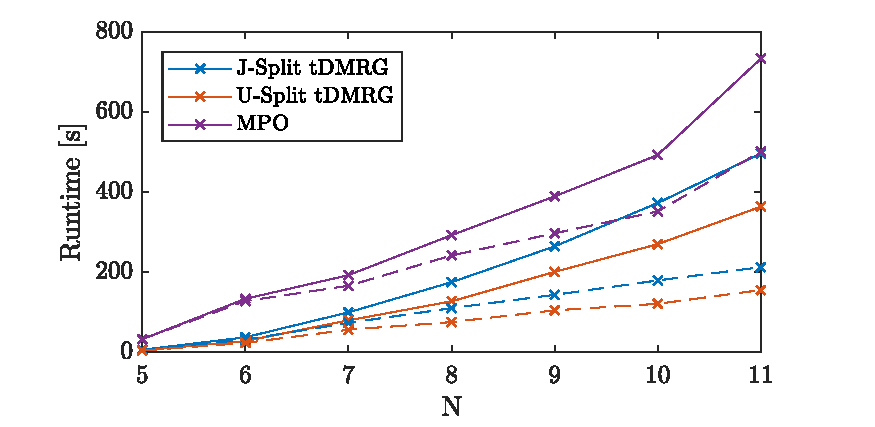
\includegraphics[width=0.7\textwidth]{Figures/CompareRuntime.pdf}
    \caption{\textit{Runtime of performing 100 time steps with various algorithms in Bose Hubbard system with unit occupancy. Solid lines are systems with a local Fock space of dimension $N$, while dashed lines are systems with a constant Fock space dimension of 5.}}
    \label{fig:CompareRuntime}
\end{figure}
A comparison between the run-times of various time-evolution algorithms in shown in Figure \ref{fig:CompareRuntime}. The two tDMRG algorithms are the one described above using a half-step of $\hat{\mathcal{U}}_{J}$ and $\hat{\mathcal{U}}_{U}$ respectively. The MPO-based algorithm builds the propagator using ITensor library methods following \cite{Pollmann2015}, and the resulting MPO is applied to the MPS according to eq. \eqref{eq:optBracketsMPO}. This method has an error of order $O(\Delta t ^2)$, which is less accurate than the second-order Trotter expansion.
In Section \ref{sec:MPO} the cost of applying an MPO to an MPS was given by $\mathrm{O}(N d^2 D_W ^2 D^2)$. Considering the single-site tensors of the tDMRG algorithms, $D_W$ is zero. Since $d = N$ for the solid lines in Figure \ref{fig:CompareRuntime}, the runtime of the algorithm will have a cubic scaling with the system size. However, a much better scaling can be achieved by truncating the local Hilbert space, such that $d$ is kept constant resulting in a runtime scaling linearly with the system size.
Consider the case of the Bose Hubbard model, eq. \eqref{BHhamil}. The interaction term scales quadratically with the number of particles at a given site, which causes a huge energy penalty even in low end of the tight binding limit. Thus, for large systems with unit occupation, neglecting contributions from states with a majority of the particles at a single site is a reasonable approximation.
Therefore, the modified tDMRG algorithm can be applied to very large systems at a low cost, if the dimension of the physical index of the MPS is restricted to a reasonable fraction of the number of particles.   